\begin{frame}
      \frametitle{Analyzing Probabilistic/Approximate VLSI Design}
      \begin{itemize}
            \item Partial design problem~\cite{Gitina2013} of probabilistic design
                  \begin{itemize}
                        \item Synthesize black-box outputs $T$ to realize specification
                        \item \alert{Constraints on inputs} to black boxes: $D_i \subseteq X \cup Y$
                  \end{itemize}
      \end{itemize}
      \begin{figure}
            \centering
            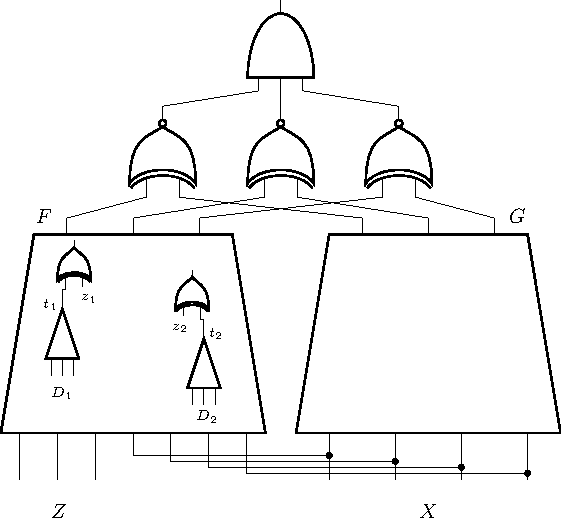
\includegraphics[scale=0.6]{fig/dependency-ssat/dssat-prob-miter.pdf}
      \end{figure}
      \begin{align*}
            \random{} X,\random{} Z,\forall Y,\exists T(D).
            (Y \equiv E(X)) \limply (F(X,Z,T) \equiv G(X))
      \end{align*}
\end{frame}